\documentclass{standalone}
 
\usepackage{tikz}
\usetikzlibrary{automata,positioning}
 
\begin{document}
    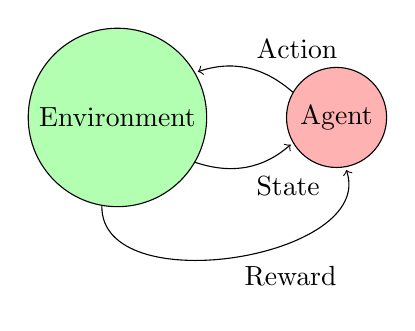
\begin{tikzpicture}
        % Draw the states
        \node[state, fill=green!30] (s) {Environment};
        \node[state, right=of s, fill=red!30] (r) {Agent};
 
        % Connect the states with arrows
        \draw[every loop]  
		(s) edge[bend right, auto=right]  node {State} (r)
		(s) edge[bend right=100, auto=right]  node {Reward} (r)		
		(r) edge[bend right, auto=right] node {Action} (s);

    \end{tikzpicture}
\end{document}